\documentclass[tikz,border=4pt]{standalone}
\usepackage[T1]{fontenc}
\usepackage{mathptmx}
\usetikzlibrary{arrows.meta,calc}
\begin{document}
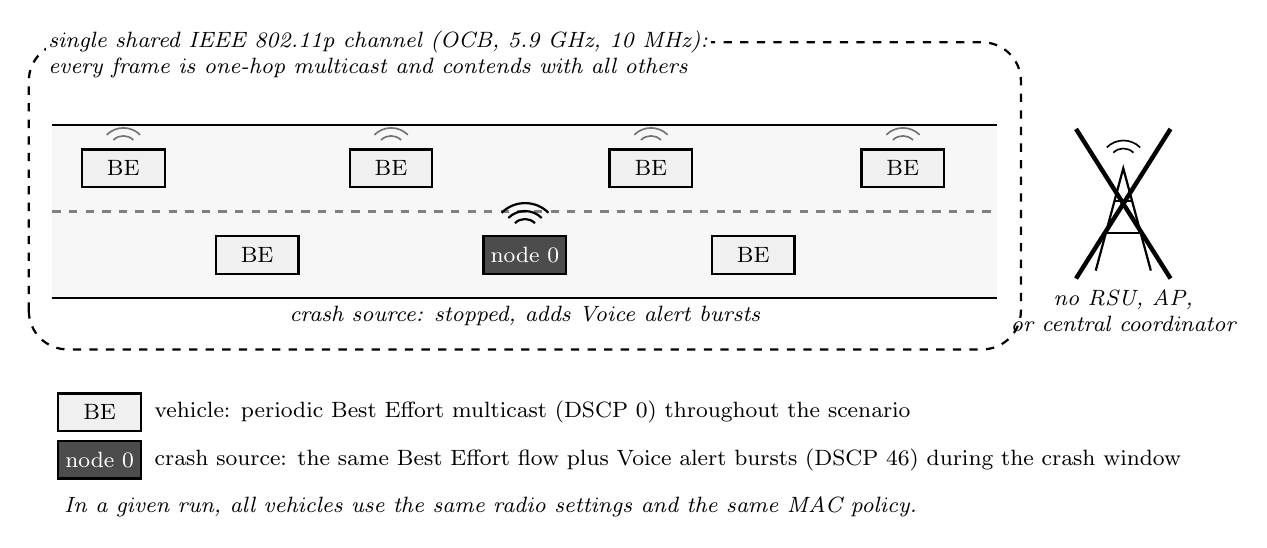
\begin{tikzpicture}[
  font=\small,
  >=Stealth,
  thick,
  car/.style={draw, thick, fill=black!6, minimum width=1.05cm, minimum height=0.48cm, inner sep=0pt, font=\footnotesize},
  crash/.style={car, fill=black!70, text=white},
  lab/.style={font=\footnotesize\itshape, align=center, inner sep=1pt},
  box/.style={draw, thick, align=left, inner sep=4pt, font=\scriptsize},
]

  % ===== Shared channel (one-hop multicast domain) =====
  \draw[thick, dashed, rounded corners=14pt] (-0.3,-0.35) rectangle (12.3,3.55);
  \node[lab, anchor=north west, align=left, fill=white] at (-0.1,3.75)
    {single shared IEEE~802.11p channel (OCB, 5.9~GHz, 10~MHz):\\every frame is one-hop multicast and contends with all others};

  % ===== Road =====
  \fill[black!3] (0,0.3) rectangle (12,2.5);
  \draw[thick] (0,0.3) -- (12,0.3);
  \draw[thick] (0,2.5) -- (12,2.5);
  \draw[thick, dashed, black!50] (0,1.4) -- (12,1.4);

  % background vehicles (both lanes)
  \foreach \x/\y in {0.9/1.95, 2.6/0.85, 4.3/1.95, 7.6/1.95, 8.9/0.85, 10.8/1.95}{
    \node[car] at (\x,\y) {BE};
  }
  % crash source
  \node[crash] (cv) at (6.0,0.85) {node 0};

  % radio emission marks above a few vehicles
  \foreach \x/\y in {0.9/1.95, 4.3/1.95, 7.6/1.95, 10.8/1.95}{
    \foreach \r in {0.18,0.30}{
      \draw[black!55, line width=0.6pt] ($(\x,\y)+(-\r*0.7,0.26+\r*0.55)$) arc[start angle=135, end angle=45, radius=\r];
    }
  }
  \foreach \r in {0.18,0.30,0.42}{
    \draw[line width=0.8pt] ($(cv.north)+(-\r*0.7,0.05+\r*0.55)$) arc[start angle=135, end angle=45, radius=\r];
  }
  \node[lab, anchor=north] at (6.0,0.25) {crash source: stopped, adds Voice alert bursts};

  % ===== No infrastructure =====
  \begin{scope}[shift={(13.6,1.4)}]
    \draw[thick] (-0.35,-0.75) -- (0,0.55) -- (0.35,-0.75);
    \draw[thick] (-0.22,-0.27) -- (0.22,-0.27);
    \draw[thick] (-0.12,0.13) -- (0.12,0.13);
    \foreach \r in {0.18,0.30}{
      \draw[line width=0.6pt] (-\r*0.7,0.65+\r*0.55) arc[start angle=135, end angle=45, radius=\r];
    }
    \draw[line width=1.6pt] (-0.6,-0.85) -- (0.6,1.05);
    \draw[line width=1.6pt] (-0.6,1.05) -- (0.6,-0.85);
    \node[lab, anchor=north] at (0,-0.95) {no RSU, AP,\\or central coordinator};
  \end{scope}

  % ===== Legend =====
  \node[car] (l1) at (0.6,-1.15) {BE};
  \node[lab, anchor=west, font=\footnotesize] at (1.25,-1.15) {vehicle: periodic Best Effort multicast (DSCP~0) throughout the scenario};
  \node[crash] (l2) at (0.6,-1.75) {node 0};
  \node[lab, anchor=west, font=\footnotesize] at (1.25,-1.75) {crash source: the same Best Effort flow plus Voice alert bursts (DSCP~46) during the crash window};
  \node[lab, anchor=west] at (0.1,-2.35) {In a given run, all vehicles use the same radio settings and the same MAC policy.};
\end{tikzpicture}
\end{document}
